\documentclass{beamer}
\usefonttheme{serif}
\usefonttheme{professionalfonts}
\usepackage[latin1]{inputenc}
\usepackage[T1]{fontenc}
\usepackage{hhline,bm,xspace,url}
\usepackage[expert]{lucidabr}
\renewcommand{\rmdefault}{hlhj}
\usepackage{fancyvrb}
\usepackage{url,xcolor}
\usepackage{marvosym}
\usepackage[color]{guit}
\usepackage{listings}
\lstset{frame=lines,basicstyle=\ttfamily,showspaces=true,prebreak={\Righttorque},postbreak={\Lefttorque},breaklines}
\newcommand{\tl}{\TeX~Live}
\newcommand{\tpm}{\texttt{tpm}}
\newcommand{\tpms}{\tpm{}s}
\newcommand{\tlpsrc}{\texttt{tlpsrc}}
\newcommand{\tlpsrcs}{\tlpsrc{}s}
\newcommand{\tlpobj}{\texttt{tlpobj}}
\newcommand{\tlpobjs}{\tlpobj{}s}
\newcommand{\tlpdb}{\texttt{tlpdb}}
\newcommand{\tlpdbs}{\tlpdb{}s}
\newcommand{\acro}[1]{\textsc{\MakeLowercase{#1}}}
\newcommand{\ctan}{\acro{CTAN}}
\newcommand{\cmd}[1]{\textsf{#1}}
\newcommand{\button}[1]{\textsf{#1}}
\newcommand{\var}[1]{\textsl{#1}}
\newcommand{\tlmgr}{\TeX~Live Manager}
\newcommand{\XeTeX}{Xe\TeX}

\def\bigit{\\[\bigskipamount]}
\def\medit{\\[\medskipamount]}

\hyphenation{infra-struc-ture}
\DefineShortVerb{\|}

\usetheme[headheight=10pt,footheight=10pt]{boxes}
\setbeamercolor*{black on white}{bg=white,fg=black}
%\setbeamerfont*{black on white}{series=\scshape}
\addfootbox{black on white}{\hbox{\vbox to 10pt{\hspace{3em}Norbert 
Preining, \tl~2008 and the \tl~Manager -- {\normalfont\guitmeeting 2007}
 \hfill \insertframenumber\hspace{3em}~~\vfill}}}
\addheadbox{black on white}{\hbox{\vbox to 10pt{~~~\hfill\leavevmode\vfill}}}
\setbeamertemplate{navigation symbols}{}

\setlength{\parskip}{\medskipamount}

\def\cred#1{{\color{red}#1}}
\def\prog#1{\texttt{#1}}

%%%%%%%%%%%%%%%%%%%%%%%%%%%%%%%%%%%%%%%%%%%%%%%%%%%%%%%%%%%%%%%%%%
%
% here begins the stuff
%
%%%%%%%%%%%%%%%%%%%%%%%%%%%%%%%%%%%%%%%%%%%%%%%%%%%%%%%%%%%%%%%%%%%%
\title{\tl~2008 and the \tl~Manager}
\author{Norbert Preining}
\institute{Vienna University of Technology, Austria}
\date{\textsc{{\normalfont\guitmeeting*}~2008}

Pisa, Italia \hspace{\bigskipamount} 18~October 2007}

\begin{document}

\frame{\titlepage}


\begin{frame}
  \frametitle{Properties of the \tl\ distribution}

  \begin{itemize}
  \item includes all the free stuff from \textsc{ctan}
  \item ready for ``consumption'', i.e., runs from \textsc{dvd}, but
    can also installed into the file system
  \item available for a wide range of platform--operating system
    combinations
  \item currently is replacing te\TeX\ in many (Unix) distributions as
    default \TeX\ system
  \end{itemize}
\end{frame}

\begin{frame}
  \frametitle{Upstream organization}
  \begin{itemize}
  \item \textsc{svn} repository where many people have write permissions
  \end{itemize}

  \pause
  \cred{\huge STOP}

  \medskip
  \pause
  That was last year's talk \ldots
\end{frame}


\begin{frame}
  \frametitle{The new installer}
  \begin{itemize}
  \item Installation from the Internet\\
    \uncover<2-2>{or from a rsync of the archive, or from the svn
    checkout, (or from an installation)}
  \item Text and \acro{GUI} mode\\
    \uncover<3-3>{text mode emulates former shell installer, also in
    \acro{W32}, \acro{GUI} for all platforms}
  \item Windows == Unix (\emph{cum grano salis})\\
    \uncover<4-4>{text and \acro{GUI} mode, -sys vs. user mode, same
    texmf.cnf file}
  \end{itemize}
\end{frame}


\begin{frame}
  \frametitle{Where to start}
  \begin{itemize}
  \item Go and get it at
    \url{http://mirror.ctan.org/systems/texlive/tlnet/2008}\\
    ~~
  \item \Verb+install-tl-unx.tar.gz+ for Unix-ish systems\\
    ~~
  \item \Verb+install.zip+ for all systems\\
    \uncover<2-2>{supports all systems, but ships Perl for \acro{W32}}
  \item \acro{W32}: double-click the \url{.bat} file\\
    \uncover<3-3>{or start it from a cmd shell for additional arguments}
  \item Unix: \url{./install-tl}\\
    \uncover<4-4>{and add arguments if you need them}
  \end{itemize}
\end{frame}


\begin{frame}
  \frametitle{Arguments for the Installer}
  \begin{itemize}
  \item \url{-location} installation source, can be\\
    \url{/normal/path}\\
    \url{file:/some/path}\\
    \url{ftp://some.server/path}\\
    \url{http://some.server/path}
    \bigit
  \item \url{-gui} tries to start the \acro{GUI} installer,
    \url{-no-gui} for \acro{W32} to disable the default \acro{GUI}
    installer \bigit
  \item \url{-lang} specifies a language code, currently supported:
    en, de, fr, it, nl, pl, sl, zh\_cn, zh\_tw
  \item some more: \url{-profile}, \url{-non-admin}, \ldots
  \end{itemize}
\end{frame}

\begin{frame}
  \frametitle{Demo Text and \acro{GUI} mode installer}
  \begin{tabular}{ll}
  \resizebox{0.5\columnwidth}{!}{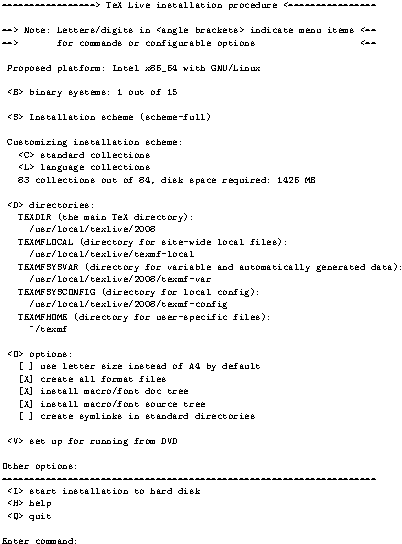
\includegraphics{install08text-crop}}
  &
 \resizebox{0.5\columnwidth}{!}{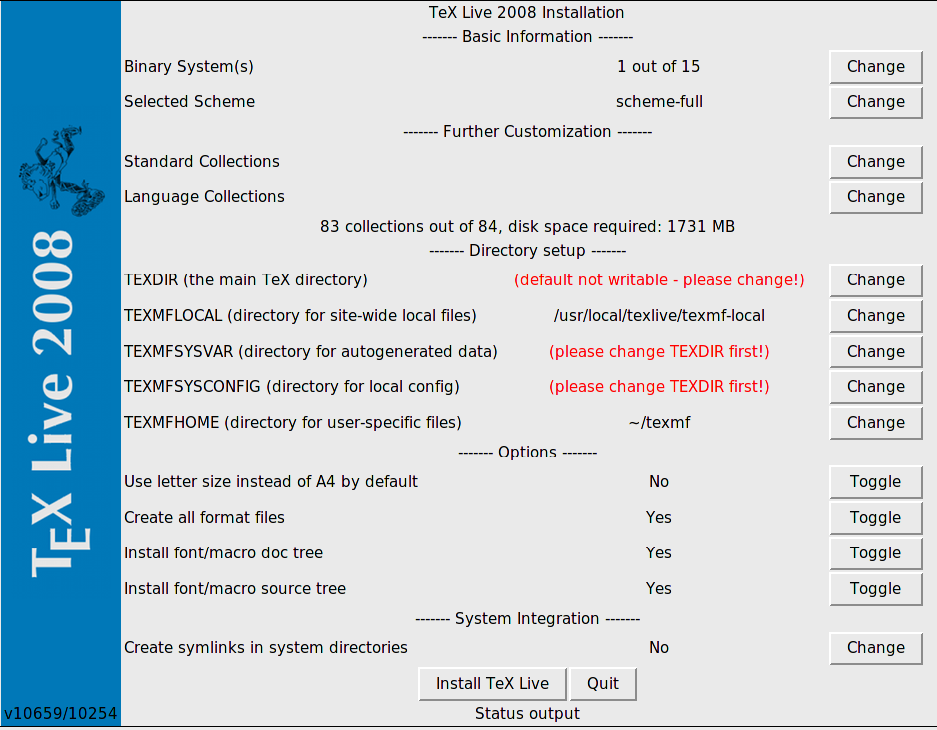
\includegraphics{gui-installer.png}}
  \end{tabular}
\end{frame}

\begin{frame}
  \frametitle{The \tlmgr}
  Syntax:
  \begin{center}
    \texttt{tlmgr \alt<2>{\cred{[opt]...}}{[opt]...} \alt<3>{\cred{action}}{action} [opt]... [arg]...}
  \end{center}
  \only<2>{
  With first set of options:
  \begin{itemize}
  \item \url{-location} installation source, see above
  \item \url{-gui} starts the \acro{GUI}
  \item \url{-gui-lang} should be auto-detected, can be overridden
  \item standard options \url{-help}, \url{-q}, \url{-v},
    \url{-version} 
  \end{itemize}
  }
  \only<3>{
  \begin{itemize}
  \item general actions: search, show, list, uninstall, check, gui,
    version, help\bigit
  \item configuration actions: option, paper, generate, uninstall\bigit
  \item package management actions: install, update, remove, backup,
    restore, arch
  \end{itemize}
  }
\end{frame}

\begin{frame}
  \frametitle{The search (and show) action}
  \begin{center}
    \texttt{tlmgr [opt]... search \cred{[opt]... what}}
  \end{center} 
  searches the \emph{locally} installed package names and descriptions
  for \texttt{\cred{what}}.

  Options:
  \begin{itemize}
  \item \texttt{-global} also searches the remote database
  \item \texttt{-file} searches for file names
  \end{itemize}
  \pause
  \begin{center}
    \texttt{tlmgr [opt]... show \cred{what}}
  \end{center} 
  shows information on the given packages
  
  \pause
  Demo
\end{frame}

\begin{frame}
  \frametitle{The install action}
  \begin{center}
    \texttt{tlmgr [opt]... install \cred{[opt]... what}}
  \end{center} 
  installs the package \texttt{what} including all dependencies

  Options:
  \begin{itemize}
  \item \texttt{-no-depends} do not install dependencies
  \item \texttt{-no-depends-at-all} do not even install architecture
    specific sub-packages
  \end{itemize}

  \pause
  Demo
\end{frame}

\begin{frame}
  \frametitle{The update action}
  \begin{center}
    \texttt{tlmgr [opt]... update \cred{[opt]... what}}
  \end{center} 
  installs the package \texttt{what} including all dependencies

  Options:
  \begin{itemize}
  \item \texttt{-list} list packages to be updated (or added) with
    revisions 
  \item \texttt{-all} update everything
  \item \texttt{-dry-run} don't actually do it
  \item \texttt{-backupdir dir} saves a snapshot of the current status to
    the specified directory
  \item \texttt{-no-depends}, \texttt{-no-depends-at-all} as before
  \end{itemize}

  \pause
  Demo
\end{frame}


\begin{frame}
  \frametitle{The \acro{GUI} of the \tlmgr}
  
  \begin{figure}[ht!]
    \centering
    \resizebox{\columnwidth}{!}{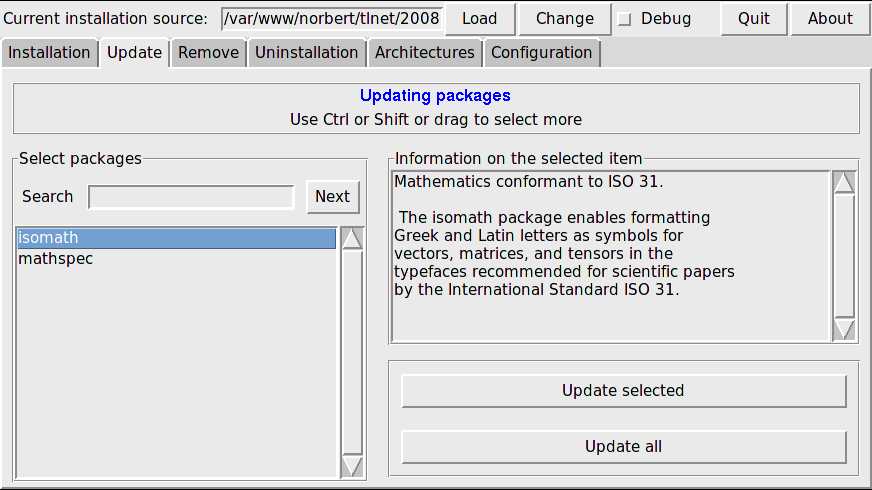
\includegraphics{tlmgrgui-update.png}}
  \end{figure}

  Demo
\end{frame}

\begin{frame}
  \frametitle{What else -- Windows}
  \begin{description}
  \item[Perl and Ghostscript.] `hidden' copies, no interference with
    full-scale distributions\bigit
  \item[\texttt{fc-cache}] helps \XeTeX{} to handle fonts more
    efficiently.\bigit
  \item[PS\_View.] a new PostScript (and \acro{PDF} viewer
    that is free software\bigit
  \item[dviout] \acro{DVI} previewer
  \end{description}
\end{frame}

\begin{frame}
  \frametitle{Really new -- Windows \acro{II}}
  A \tlmgr\ Updater in \.exe format
\end{frame}

\begin{frame}
  \frametitle{Closing}
  \begin{itemize}
  \item very much work in progress, please do update your tlmgr
    immediately after a new installation\bigit
    \pause
  \item the \acro{GUI} needs a lot of work, does not exhibit all the
    functionality of the cmd line version \bigit
    \pause
  \item Perl programmers -- join us!\bigit
  \end{itemize}
\end{frame}

\begin{frame}
  \begin{center}
    {\Large Thanks}

    \bigskip
    Karl Berry\\
    {\small for great enthusiasm and  perpetual
      support (and critical voices)}
    
    \pause
    \bigskip
    \acro{TUG} and \acro{DANTE}\\
    {\small for financial support when my laptop broke}
    
    \pause
    \bigskip
    Your Attention
  \end{center}
\end{frame}
\end{document}
